\documentclass{article}
\usepackage{graphicx} % Required for inserting images
\usepackage{pifont}
\usepackage[utf8]{inputenc}
\usepackage{amsmath}
\usepackage{listings}

\usepackage{xcolor}
\usepackage{mdframed}

\definecolor{light-gray}{gray}{0.95}
\newcommand{\code}[1]{\colorbox{light-gray}{\texttt{#1}}}
\usepackage{float} % For specifying figure positioning
\usepackage{geometry}
\geometry{margin=1in}
% \geometry{margin=1.5in}

\title{Deep Learning and Natural Language Processing Project}
\author{Moria Grohar, Shirel Zecharia}
\date{\today}

\begin{document}

\maketitle
\tableofcontents
\newpage

\section{Abstract}
In this report, we present a study on implementing a neural network model for the classification of fashion items using the Fashion MNIST dataset.\\
We compare the performance of the neural network approach with traditional machine learning algorithms such as Logistic Regression, and Multi-Layer Perceptron (MLP).\\
The report discusses the project methodology, experimental results, and conclusions drawn from the comparison.

\section{Introduction}
This report explores the performance of various machine learning models for classifying fashion items from the well-known Fashion-MNIST dataset. This dataset consists of grayscale images of various clothing articles, each belonging to a specific category such as T-shirts, trousers, and shoes. The task of classifying these images is considered a classification problem.

The report delves into the implementation and evaluation of different models,
including several models from sklearn, neural network from tensorflow and CNN.

The models were evaluated based on their loss function, with the aim of achieving the lowest possible loss to indicate better performance in classifying the fashion items.

The report compares and analyzes the results of each model, providing insights into their strengths and weaknesses for this specific classification task. It also discusses potential areas for further exploration and improvement.

\section{Related Work and Required Background}
\subsection{Softmax Regression}
Softmax regression, also known as multinomial logistic regression, is a generalization of logistic regression.
While in logistic regression we assumed that the labels were binary: ${y(i)\in{0,1}}$, In Softmax regression we are able to handle multiple labels ${y(i)\in{1,…,K}}$ where ${k}$ is the number of classes.\\

In softmax regression, the goal is to predict the probability that an input sample belongs to each possible class. This is achieved by applying the softmax function to the output of a linear model. The linear model computes a score for each class based on the input features, and the softmax function converts these scores into probabilities.\\

Mathematically, given an input vector ${x}$, softmax regression computes the probability ${P(y=i | x)}$ that the input belongs to class ${i}$ as follows:
$${P(y=i | x) = \frac{e^{x^{T} \cdot W_i + b_i}}{\sum_{j=1}^{k} e^{x^{T} \cdot W_j + b_j}}
        }$$

\noindent\hspace*{10mm}
\begin{minipage}{\dimexpr\linewidth-20mm}
    Where:\\
    ${y}$ is the target variable (class).\\
    ${x}$ is the vector of input features.\\
    ${T}$ denotes the transpose applied to the vector.\\
    ${W_i}$: the weight vector associated with class ${i}$.\\
    ${b_i}$: the bias term associated with class ${i}$.\\
\end{minipage}\\
\textbf{Understanding The Process:}\hfill\newline\\
Linear Transformation: For each class, it computes a linear combination of the input features using class-specific weights. This generates a score for each class, indicating its "fit" for the data point.\hfill\newline\\
Softmax Function: This function takes the vector of scores and transforms them into probabilities. It ensures:
\begin{itemize}
    \item Non-negativity: All probabilities are positive (between 0 and 1).
\end{itemize}
\begin{itemize}
    \item Normalization: The sum of all probabilities for a single data point is always 1, representing a valid probability distribution.
\end{itemize}
The softmax function is often used as the final activation layer in multi-class neural networks as we will discuss later in the article.

\subsection{Activation Functions}
Activation functions are mathematical functions used to determine the output of a neuron, influencing how information flows through the network and ultimately shaping its learning and decision-making capabilities.\\\\
Traditional neural networks without activation functions would simply perform linear transformations on the input data. This limitation restricts them from learning complex patterns and relationships in the data, hindering their ability to perform tasks like image recognition or natural language processing.\\\\
A neuron in a neural network receives multiple inputs, each carrying a specific value. These inputs are combined through weighted connections and then passed through an activation function. The function acts like a filter, transforming the combined input into a single output value. This output value then becomes the basis for the neuron's activation, influencing the signals it transmits to other neurons in the network.\\\\
The selection of an appropriate activation function depends on the specific task and network architecture. While ReLU and Leaky ReLU are popular choices due to their efficiency, other functions like sigmoid and tanh might be suitable for specific scenarios like output normalization or recurrent neural networks.\newline\newline
\textbf{Popular Activation Functions:}\hfill\newline

\begin{itemize}
    \item[\ding{118}] Rectified Linear Unit:
          ReLU (Rectified Linear Unit) activation functions serve as the non-linear activation function of choice in most CNN architectures. ReLU introduces non-linearity into the network, enabling it to learn complex mappings between the input and output. Mathematically, ReLU simply outputs the input if it is positive and zero otherwise, which simplifies computations and accelerates convergence during training.
\end{itemize}

\begin{itemize}
    \item[\ding{118}] Leaky Rectified Linear Unit:
          Leaky ReLU is a variant of the ReLU activation function that addresses the "dying ReLU" problem, where neurons may become inactive and cease to update their weights during training. Unlike ReLU, which sets negative values to zero, Leaky ReLU allows a small, non-zero gradient for negative inputs. This modification ensures that neurons remain active and continue to contribute to the learning process, especially in deeper networks where vanishing gradients are more prevalent.
\end{itemize}

\begin{itemize}
    \item[\ding{118}] Sigmoid:
          This function squishes the input values between 0 and 1, mimicking the firing behavior of biological neurons. However, its vanishing gradients can hinder learning in deep networks.
\end{itemize}

\begin{itemize}
    \item[\ding{118}] Tanh (Hyperbolic tangent):
          Similar to sigmoid, tanh maps the input values to a range of -1 to 1. It offers slightly better gradients than sigmoid but suffers from similar limitations.
\end{itemize}
\newpage

\subsection{Simple Neural Networks}
A simple neural network consists of interconnected neurons organized in layers. Each neuron calculates a weighted sum of its inputs, applies an activation function and passes the result on to the next layer.
\subsubsection{Mathematical Representation}

Let:
\begin{itemize}
    \item \( x \) be the input vector,
    \item \( W \) be the weight matrix,
    \item \( b \) be the bias vector,
    \item \( f \) be the activation function,
    \item \( z \) be the weighted sum of inputs,
    \item \( a \) be the output after applying the activation function.
\end{itemize}

For a single neuron in a layer, the computation can be represented as:
\begin{align*}
    z & = Wx + b \\
    a & = f(z)
\end{align*}
With multiple neurons in a layer, the calculations are performed in parallel, resulting in matrix multiplication for the weighted sum and the element-wise application of the activation function.

\subsubsection{Forward Propagation}
In forward propagation, the input data is fed into the network and the calculations are performed layer by layer until the final output is obtained.
\begin{enumerate}
    \item \textbf{Input Layer}: The input data \( x \) is fed into the network.
    \item \textbf{Hidden Layers}: Each hidden layer computes the weighted sum of inputs and applies the activation function to produce the output.
    \item \textbf{Output Layer}: The final hidden layer's output is passed through the output layer, which produces the network's prediction.
\end{enumerate}
Mathematically, forward propagation can be expressed as:
\begin{align*}
    z^{[l]} & = W^{[l]}a^{[l-1]} + b^{[l]} \\
    a^{[l]} & = f(z^{[l]})
\end{align*}
where \( l \) denotes the layer index.
\subsubsection{Backpropagation}

Backpropagation is used to update the weights and biases of the network to minimize the loss function. Gradients are calculated and the parameters are adjusted using gradient descent.

The most important equations for backpropagation are the chain rule for calculating the gradients and the equations for updating the weights and biases:
\begin{align*}
    \frac{\partial \mathcal{L}}{\partial z^{[l]}} & = \frac{\partial \mathcal{L}}{\partial a^{[l]}} \cdot \frac{\partial a^{[l]}}{\partial z^{[l]}} \\
    \frac{\partial \mathcal{L}}{\partial W^{[l]}} & = \frac{\partial \mathcal{L}}{\partial z^{[l]}} \cdot \frac{\partial z^{[l]}}{\partial W^{[l]}} \\
    \frac{\partial \mathcal{L}}{\partial b^{[l]}} & = \frac{\partial \mathcal{L}}{\partial z^{[l]}} \cdot \frac{\partial z^{[l]}}{\partial b^{[l]}}
\end{align*}
where \( \mathcal{L} \) represents the loss function.

\subsection{Convolutional Neural Networks}
Convolutional Neural Networks (CNNs) are a specific type of artificial neural network architecture particularly well-suited for analyzing image data. They excel at tasks like image classification, object detection, and image segmentation. Unlike traditional neural networks, CNNs incorporate an additional layer type called a convolutional layer to extract features from the input data. The essence of a CNN lies in its ability to automatically learn spatial hierarchies of features from raw data. These networks consist of several layers, typically including convolutional layers, pooling layers, and fully connected layers.

\subsubsection{Convolutional Layers}
Convolutional layers are the cornerstone of CNNs, responsible for learning and detecting patterns within the input data. They employ mathematical operations known as convolutions to extract features such as edges, textures, and other distinctive attributes from the input images. Mathematically, convolution involves sliding a filter or a kernel over the input data, performing element-wise multiplications, and summing the results to produce feature maps.

\subsubsection{Pooling Layers}
Pooling layers reduce the spatial dimensions of feature maps generated by convolutional layers while retaining important information. Common pooling techniques include max pooling and average pooling, where the former selects the maximum value from a region of the feature map, while the latter computes the average. Pooling helps in achieving translation invariance and reducing the computational burden by downsampling the feature maps.

\subsubsection{Fully Connected Layers}
These layers function similarly to traditional neural networks, connecting all neurons in one layer to all neurons in the next. They process the extracted features and learn complex relationships to form the final output, such as a class prediction or a set of bounding boxes for object detection.

\subsection{Optimizers}
Optimizers are used for updating the model's parameters to minimize the loss function during the training process, which ultimately leads to better performance of the model.

\subsubsection{Stochastic Gradient Descent (SGD)}
The SGD algorithm takes a single data point (or a small batch) at a time, calculates the gradient (the direction of steepest descent in the loss function), and updates the model's parameters in the opposite direction by a small learning rate. This technique is computationally inexpensive, making it suitable for large datasets. But on the other hand it may require many iterations to reach an optimal solution, especially for complex models and datasets.\\
The update rule for SGD can be represented as:
$${\theta_{t+1} = \theta_t - \eta \cdot \nabla L(\theta_t)}$$

\noindent\hspace*{10mm}
\begin{minipage}{\dimexpr\linewidth-20mm}
    Where:\\
    ${\theta_t}$ is the current parameter values.\\
    ${\eta}$ is the learning rate, a small positive scalar determining the step size.\\
    ${\nabla L(\theta_t)}$ is the gradient of the function ${L}$ at ${\theta_t}$, which points in the direction of the steepest increase in ${L}$.
\end{minipage}

\subsubsection{Momentum SGD}
SGD with Momentum is used to improve the performance of the neural network. accelerates convergence, especially in the context of high curvature, small but consistent gradients, or noisy gradients. It does this by adding a fraction ${\gamma}$ of the update vector of the past time step to the current update.\\
The update rule for Momentum SGD is:
\begin{align*}
    v_{t}        & = \gamma \cdot v_{t-1} + \eta \nabla L(\theta_t) \\
    \theta_{t+1} & = \theta_t - v_{t}
\end{align*}

\noindent\hspace*{10mm}
\begin{minipage}{\dimexpr\linewidth-20mm}
    Where:\\
    $v_{t}$ is the velocity at time step ${t}$, which is a combination of the current gradient and the velocity from the previous step $v_{t-1}$.\\
    ${\gamma}$ (often set between 0.9 and 0.99) is the momentum term, determining how much of the past velocity to add to the current step.
\end{minipage}

\subsubsection{RMSprop (Root Mean Square Propagation)}
RMSprop addresses a limitation of SGD, where frequent updates based on noisy gradients can lead to slow convergence.
Its key Feature is that it incorporates an exponential moving average of the squared gradients for each parameter. This averages the recent updates and reduces the impact of large, infrequent gradients, leading to smoother convergence. This technique has an increased computational cost compared to SGD and RMSprop.This technique has an increased computational cost compared to SGD.

\begin{align*}
    s_{t+1}      & = \beta \cdot s_t + (1 - \beta) \cdot (\nabla L(\theta_t))^2                 \\
    \theta_{t+1} & = \theta_t - \frac{\eta}{\sqrt{s_{t+1}} + \epsilon} \cdot \nabla L(\theta_t)
\end{align*}

\subsubsection{Adam (Adaptive Moment Estimation)}
The Adam optimizer combines ideas from SGD, RMSprop, and momentum, aiming to adapt the learning rate for each parameter individually and accelerate convergence.
It maintains exponential moving averages of gradients (similar to RMSprop) and squared gradients.
It incorporates momentum to account for the history of past updates, addressing the issue of getting stuck in local minima.
It adaptively adjusts the learning rate for each parameter based on these estimates, aiming for optimal updates. This technique has an increased computational cost compared to SGD and RMSprop.
\begin{align*}
    m_{t+1}       & = \beta_1 \cdot m_t + (1 - \beta_1) \cdot \nabla L(\theta_t)                  \\
    v_{t+1}       & = \beta_2 \cdot v_t + (1 - \beta_2) \cdot (\nabla L(\theta_t))^2              \\
    \hat{m}_{t+1} & = \frac{m_{t+1}}{1 - \beta_1^{t+1}}                                           \\
    \hat{v}_{t+1} & = \frac{v_{t+1}}{1 - \beta_2^{t+1}}                                           \\
    \theta_{t+1}  & = \theta_t - \frac{\eta}{\sqrt{\hat{v}_{t+1}} + \epsilon} \cdot \hat{m}_{t+1}
\end{align*}

\newpage
\section{Previous Attempts}
\subsection{First Attempts with different data}
Model Selection and Evaluation:

The project explored the performance of various models for predicting flight ticket prices in a dataset containing information on bookings between major Indian cities. The target variable was the "Price" column, indicating a continuous value. Therefore, the problem was classified as a regression task.

The data was split into train and test sets for model evaluation. Several models were implemented and compared based on their performance in reducing the mean squared error (MSE), which served as the loss function.\\

\textbf{Model Performances:}\\


\subsubsection{Dummy Model:}
This baseline model adopted a simple mean strategy, resulting in high loss values.
\begin{figure}[H]
    \caption{Dummy model flight result:}
    \centering
    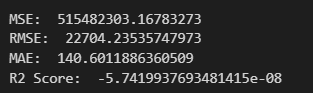
\includegraphics[width=8cm]{imgFolder/dummyModelFlight.png}
\end{figure}

\subsubsection{Linear Regression: }Compared to the dummy model, linear regression showed improvement but still yielded significant loss.
\begin{figure}[H]
    \caption{Linear Regression model flight result:}
    \centering
    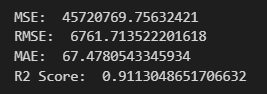
\includegraphics[width=8cm]{imgFolder/linearRegressionFlight.png}
\end{figure}

\subsubsection{Ridge Regression: }A slight reduction in loss compared to linear regression was observed, but the values remained high.
\begin{figure}[H]
    \caption{Ridge Regression model flight result:}
    \centering
    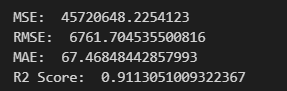
\includegraphics[width=8cm]{imgFolder/ridgeRegressionFlight.png}
\end{figure}

\subsubsection{Random Forest: }This model achieved a more significant reduction in loss compared to prior models, although the value remained high.
\begin{figure}[H]
    \caption{Random Forest model flight result:}
    \centering
    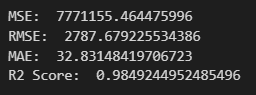
\includegraphics[width=8cm]{imgFolder/randomForestFlight.png}
\end{figure}

\subsubsection{Linear Regression with TensorFlow: }Implementing linear regression using TensorFlow did not improve performance and even resulted in higher loss compared to the basic implementation.
\begin{figure}[H]
    \caption{Linear Regression with TensorFlow model flight result:}
    \centering
    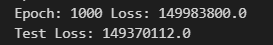
\includegraphics[width=8cm]{imgFolder/linearRegressionTensorflowFlight.png}
\end{figure}

\subsubsection{Neural Network Exploration:}

\begin{figure}[H]
    A neural network model with 2 hidden layers and 80 hidden units was constructed using TensorFlow. Hyperparameter tuning involved adjusting the learning rate and number of epochs, ultimately leading to the configuration with the lowest observed loss.
    \caption{neural network model flight result:}
    \centering
    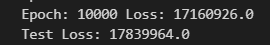
\includegraphics[width=8cm]{imgFolder/neuronNetworkFlight.png}
\end{figure}

\subsubsection{Comparison and Conclusion:}
\begin{figure}[H]
    \caption{comparison model flight result:}
    \centering
    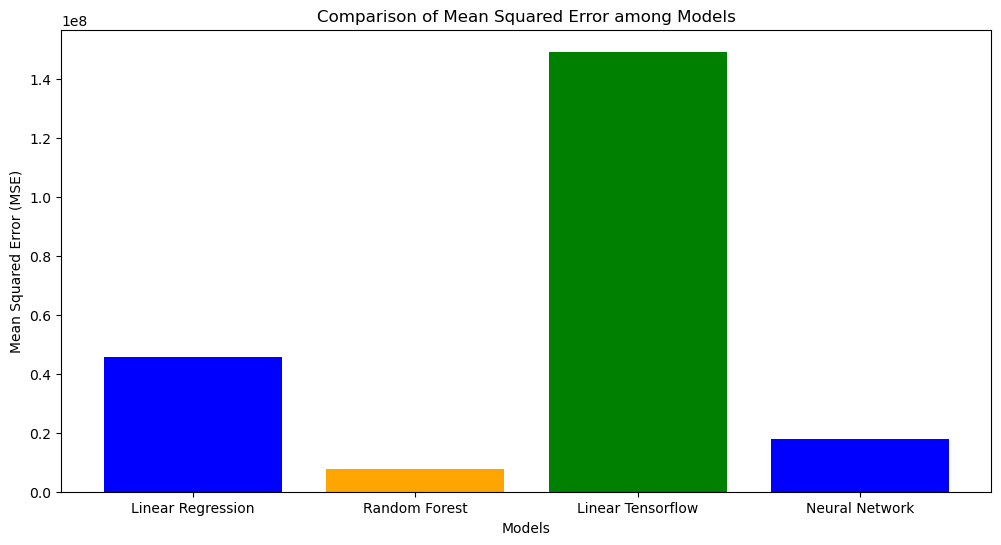
\includegraphics[width=8cm]{imgFolder/comparisonFlight.png}
\end{figure}
While the neural network achieved competitive results compared to simpler models after hyperparameter adjustments, the random forest remained the best performing model based on the achieved loss values.

\subsection{Second Attempts with Fashion-MNIST data (our data)}
\textbf{Model Selection and Evaluation:}

The project explored the performance of various models for classification of a picture of cloth to a various category. Therefore, the problem was classified as a classification task.

The data was split into train and test sets for model evaluation, in some models also to validation. Several models were implemented and compared based on their performance in reducing the loss function.\\
\textbf{Approach:}

In this study, the waterfall approach is adopted, characterized by systematically running the model with predefined epochs and various parameters governing the model's architecture, such as the number of layers in the neural network and other relevant factors. This method aims to systematically explore the model's performance across different configurations and settings.\\
\textbf{Model Performances:}\\

\subsubsection{Soft max:}
A function that turns a vector of K real values into a vector of K real values that sum to 1.

In an effort to optimize the performance of the model's performance, various hyperparameters were explored.
The number of epochs controlling the training iterations was adjusted.
Different optimizers responsible for updating the model weights were investigated. The split of data for training, validation and testing was also investigated.
The aim of this approach was to achieve the best possible result with the smallest loss function and the highest accuracy.

The accuracy calculation process.
\begin{figure}[H]
    \caption{Running the model:}
    \centering
    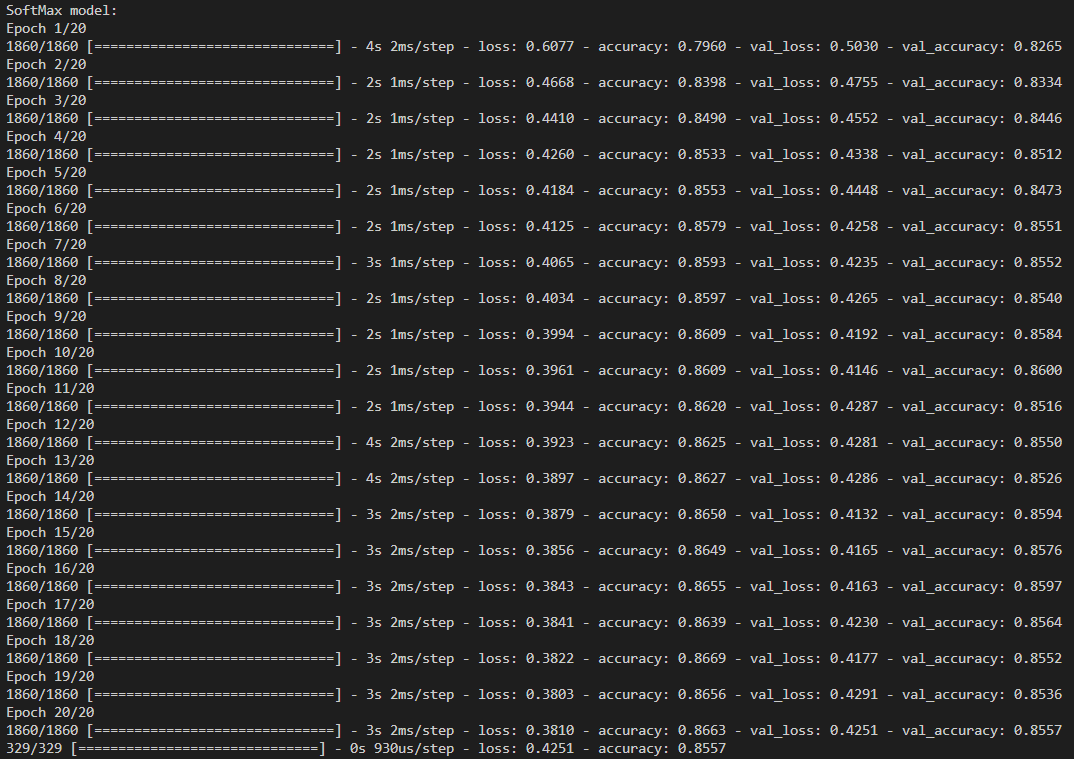
\includegraphics[width=15cm]{imgFolder/RunningSoftMax.png}
\end{figure}
The result of the run:
\begin{figure}[H]
    \caption{Result:}
    \centering
    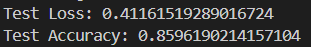
\includegraphics[width=10cm]{imgFolder/softMaxResult.png}
\end{figure}

The classification report in concentrated form:
\begin{figure}[H]
    \caption{Classification Report:}
    \centering
    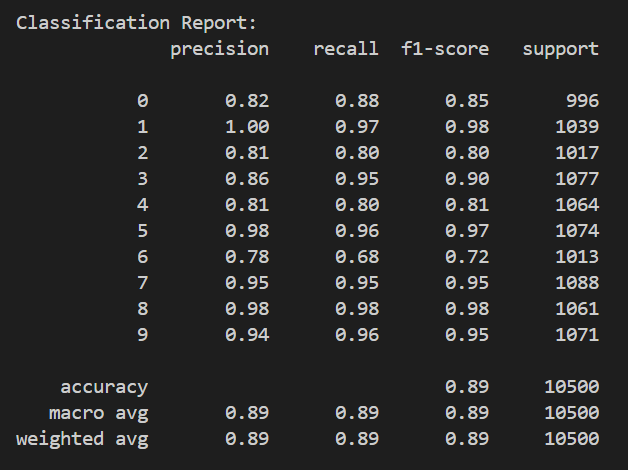
\includegraphics[width=10cm]{imgFolder/classificationReportSoftmax.png}
\end{figure}

All the data of the epochs can be shown in a graph that shows the loss function and the accuracy in every run.
\begin{figure}[H]
    \caption{Soft max training history:}
    \centering
    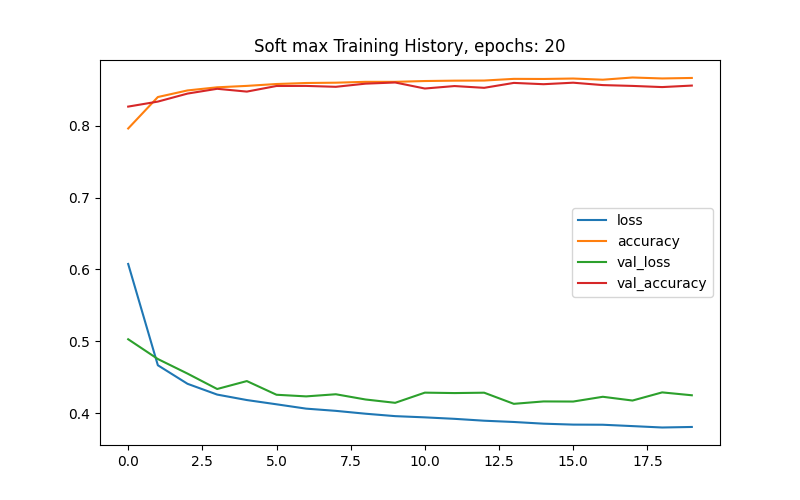
\includegraphics[width=10cm]{imgFolder/softMax_fig.png}
\end{figure}
\newpage

\subsubsection{CNN:}
A regularized type of feed-forward neural network that learns feature engineering by itself via filters (or kernel) optimization.
In an effort to optimize the performance of the model's performance, various hyperparameters were explored.
The number of epochs controlling the training iterations was adjusted. Different optimizers responsible for updating the model weights were investigated. The split of data for training, validation and testing was also investigated.
The aim of this approach was to achieve the best possible result with the smallest loss function and the highest accuracy.

The accuracy calculation process:

\begin{figure}[H]
    \caption{Running the model:}
    \centering
    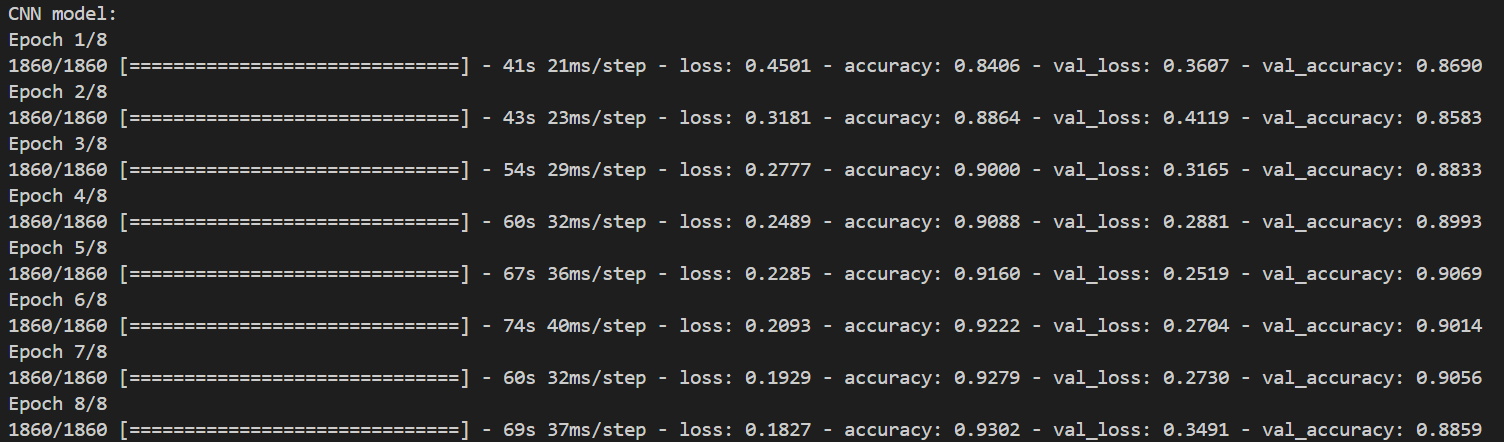
\includegraphics[width=10cm]{imgFolder/RunningCNNModel.png}
\end{figure}

The result of the run:
\begin{figure}[H]
    \caption{Result:}
    \centering
    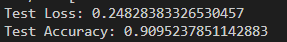
\includegraphics[width=10cm]{imgFolder/CNNResult.png}
\end{figure}

The classification report in concentrated form:
\begin{figure}[H]
    \caption{Classification Report:}
    \centering
    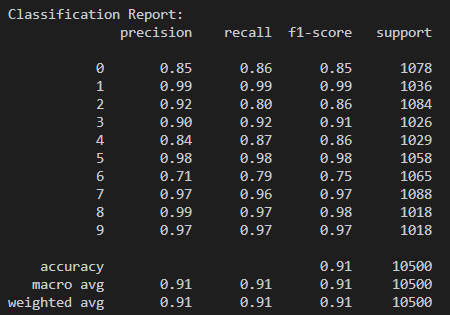
\includegraphics[width=10cm]{imgFolder/classificationReportCNN.png}
\end{figure}

All the data of the epochs can be shown in a graph that shows the loss function and the accuracy in every run.
\begin{figure}[H]
    \caption{CNN training history:}
    \centering
    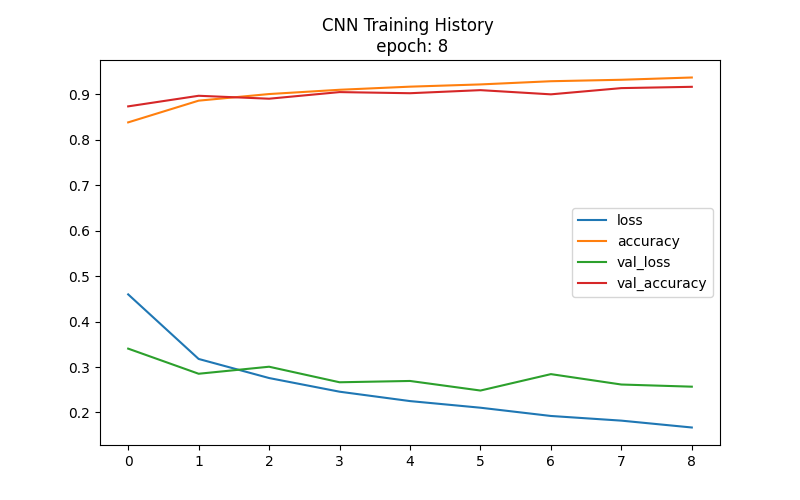
\includegraphics[width=10cm]{imgFolder/CNN_fig.png}
\end{figure}

\subsubsection{Simple Neural Network:}
A group of interconnected units called neurons that send signals to one another. Neurons can be either biological cells or mathematical models. While individual neurons are simple, many of them together in a network can perform complex tasks.In an effort to optimize the performance of the model's performance, various hyperparameters were explored.
The number of epochs controlling the training iterations was adjusted. Different optimizers responsible for updating the model weights were investigated. The split of data for training, validation and testing was also investigated.
The aim of this approach was to achieve the best possible result with the smallest loss function and the highest accuracy.

The accuracy calculation process:

\begin{figure}[H]
    \caption{Running the model:}
    \centering
    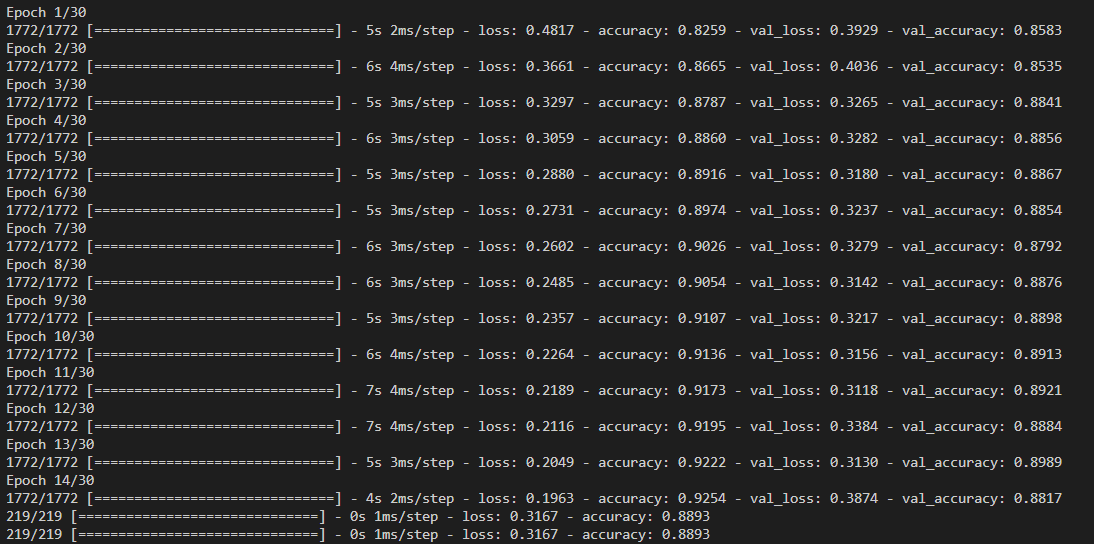
\includegraphics[width=10cm]{imgFolder/RunningSimpleNeuralNetwork.png}
\end{figure}

The result of the run:
\begin{figure}[H]
    \caption{Result:}
    \centering
    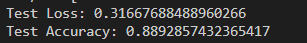
\includegraphics[width=10cm]{imgFolder/simpleNeuralNetworkResult.png}
\end{figure}

The classification report in concentrated form:
\begin{figure}[H]
    \caption{Classification Report:}
    \centering
    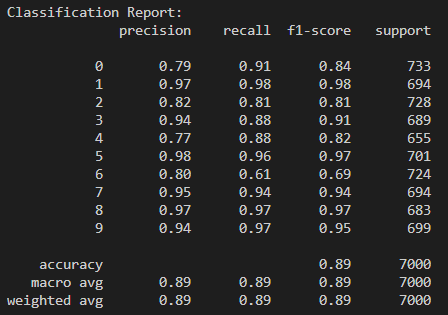
\includegraphics[width=10cm]{imgFolder/classificationReportSimpleNeuralNetwork.png}
\end{figure}

All the data of the epochs can be shown in a graph that shows the loss function and the accuracy in every run.
\begin{figure}[H]
    \caption{Simple Neural Network training history:}
    \centering
    \includegraphics[width=10cm]{imgFolder/SimpleNeuralNetwork_fig.png}
\end{figure}
\subsection{Comparing Between Models}
\begin{figure}[H]
    \caption{Comparing accuracy score between models: }
    \centering
    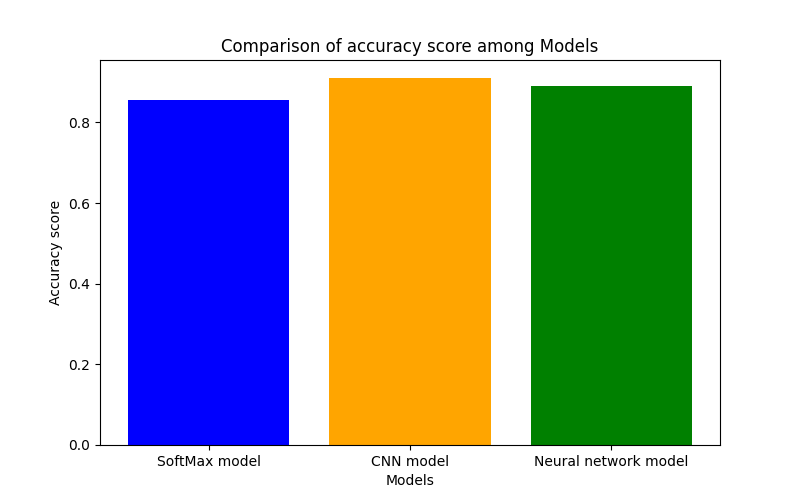
\includegraphics[width=10cm]{imgFolder/accurateFuncComparison.png}
\end{figure}
\begin{figure}[H]
    \caption{Comparing loss function between models:}
    \centering
    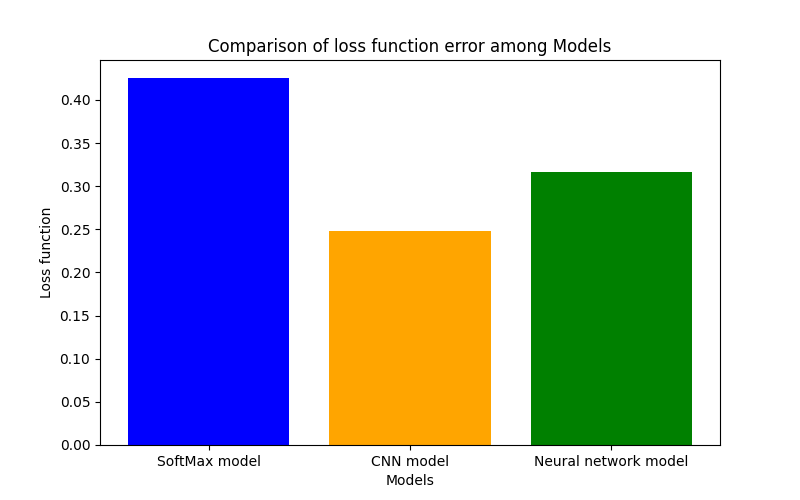
\includegraphics[width=10cm]{imgFolder/lossFuncComparison.png}
\end{figure}

The comparison shows that the CNN model has the lowest loss function and the highest accuracy among the evaluated models, indicating its superior performance.

\newpage

\section{Project Description}

The optimal model architecture determined in this study is a Convolutional Neural Network (CNN) with the following specifications:

\begin{enumerate}
    \item \textbf{input layer}:
          \begin{itemize}
              \item Convolution layer with 32 filters of size 3x3.
              \item Activation function: specified by the variable \texttt{activation}.
              \item Input shape: determined by the variable \texttt{input\_shape}.
          \end{itemize}

    \item \textbf{normalization}:
          \begin{itemize}
              \item Batch normalization layer.
          \end{itemize}

    \item \textbf{Pooling Layers}:
          \begin{itemize}
              \item MaxPooling2D layer with a pool size of 2x2.
          \end{itemize}

    \item \textbf{Convolutional Layers}:
          \begin{itemize}
              \item Another convolutional layer with 64 filters of size 3x3.
              \item Activation function: the same as specified in the variable \texttt{activation}.
          \end{itemize}

    \item \textbf{normalization}:
          \begin{itemize}
              \item Batch normalization level.
          \end{itemize}

    \item \textbf{Pooling Layers}:
          \begin{itemize}
              \item MaxPooling2D layer with a pool size of 2x2.
          \end{itemize}

    \item \textbf{Convolutional Layers}:
          \begin{itemize}
              \item Third convolutional layer with 64 filters of size 3x3.
              \item Activation function: the same as specified in the variable \texttt{activation}.
          \end{itemize}

    \item \textbf{Normalization}:
          \begin{itemize}
              \item Batch normalization layer.
          \end{itemize}

    \item \textbf{Flattening Layer}:
          \begin{itemize}
              \item Flattening layer for converting the 2D feature maps into a 1D vector.
          \end{itemize}

    \item \textbf{Dense Layers}:
          \begin{itemize}
              \item Fully connected dense layer with 64 neurons.
              \item Activation function: same as specified in the variable \texttt{activation}.
          \end{itemize}

    \item \textbf{Dropout}:
          \begin{itemize}
              \item Dropout layer with a dropout rate specified by \texttt{dropout\_rate}.
          \end{itemize}

    \item \textbf{Output Layer}:
          \begin{itemize}
              \item Dense layer with the number of neurons equal to the number of classes: 10.
              \item Activation function: softmax.
          \end{itemize}
\end{enumerate}

The result obtained by this CNN architecture is the lowest loss function and the highest accuracy among the models evaluated in the study.
The results:
\begin{enumerate}
    \item \textbf{Accuracy: } 91\%

    \item \textbf{Loss Function: } 0.25\%

\end{enumerate}

\newpage
\section{Simulation Results}

\subsection{Softmax Regression Model}

\begin{figure}[H]
    \caption{Training history of the data}
    \centering
    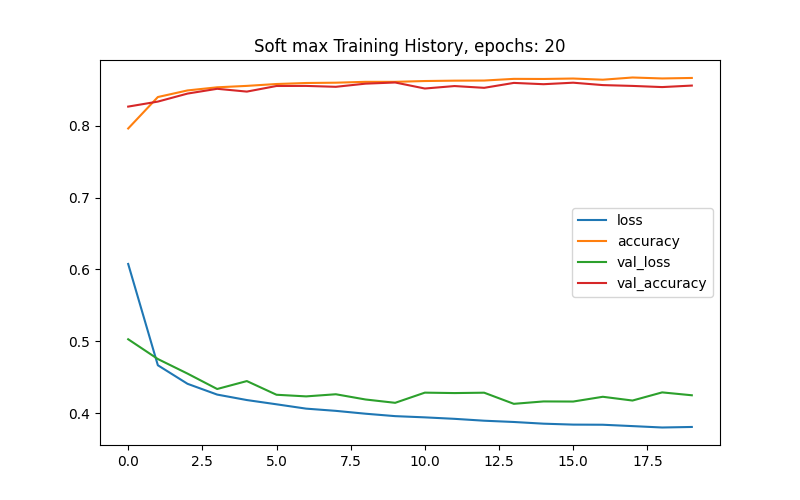
\includegraphics[width=8cm]{imgFolder/softMax_fig.png}
\end{figure}

\begin{figure}[H]
    \caption{Output}
    \centering
    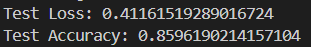
\includegraphics[width=6cm]{imgFolder/softMaxResult.png}
\end{figure}

\subsection{Simple Neural Network Model}

\begin{figure}[H]
    \caption{Training history of the data}
    \centering
    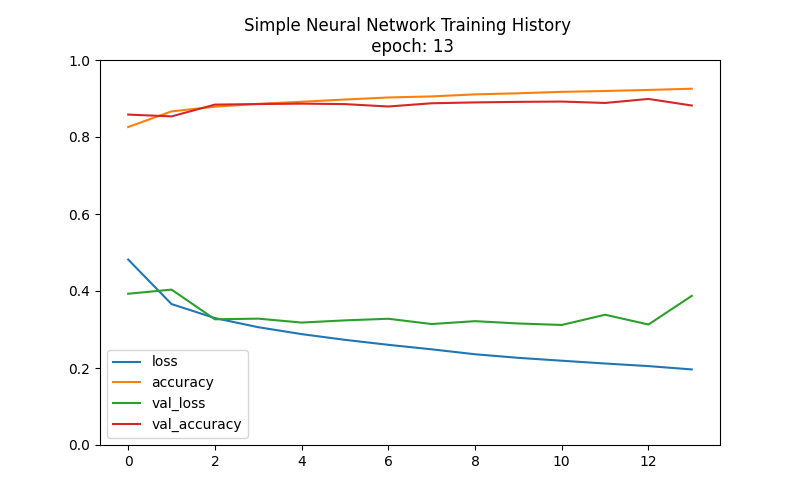
\includegraphics[width=8cm]{imgFolder/simpleNeuralNetwork_fig.png}
\end{figure}

\begin{figure}[H]
    \caption{Output}
    \centering
    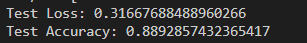
\includegraphics[width=6cm]{imgFolder/simpleNeuralNetworkResult.png}
\end{figure}

\subsection{Convolutional Neural Network Model}
\begin{figure}[H]
    \caption{Training history of the data}
    \centering
    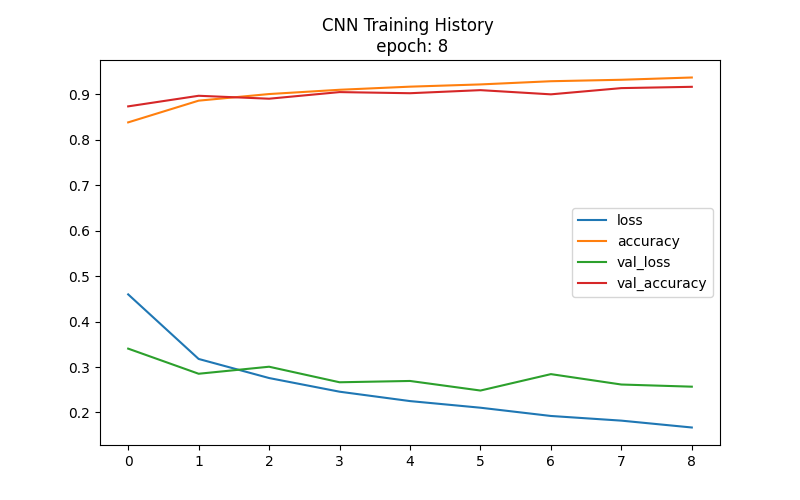
\includegraphics[width=8cm]{imgFolder/CNN_fig.png}
\end{figure}

\begin{figure}[H]
    \caption{Output}
    \centering
    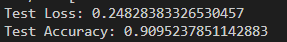
\includegraphics[width=6cm]{imgFolder/CNNResult.png}
\end{figure}

\newpage
\section{Code}
\subsection{Softmax Regression}
softMax.py implements softmax regression, a technique for multi-class classification tasks, using TensorFlow's Keras API. It comprises two functions: create-softmax-model and train-softmax-model. The former constructs a softmax regression model with a single Dense layer, which outputs class probabilities for input images. The latter function trains the model using the specified training and test data, employing the Adam optimizer and sparse categorical cross-entropy loss. The training process is visualized through a plot showcasing the model's training history (as we saw in figure 1), including loss and accuracy metrics over epochs.

\begin{figure}[H]
\caption{Creation of the Softmax model}
\centering
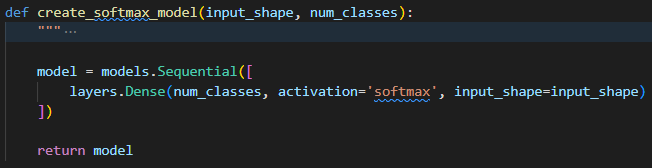
\includegraphics[width=8cm]{imgFolder/create_softmax_model.png}
\end{figure}

\begin{figure}[H]
\caption{Training of the Softmax model}
\centering
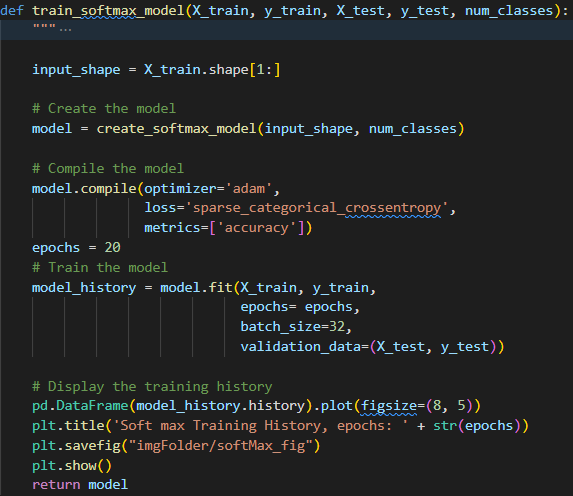
\includegraphics[width=8cm]{imgFolder/train_softmax_model.png}
\end{figure}

\newpage
\subsection{Simple Neural Network Model}
SimpleNeuralNetwork.py code implements a Simple Neural Network using TensorFlow's Keras API for image classification tasks.
It consists of three functions: split-validation, create-neural-network and train-neural-network.
The first split the data into, train, test and validation. The second, constructs a simple neural network model with multiple dense layers, along with batch normalization and dropout for regularization. The last function prepares the training and test datasets, compiles and trains the simple neural network model, and visualizes the training history, showcasing metrics evolution over epochs (as we saw in figure 10). Early stopping is used to prevent overfitting by halting training if validation loss does not improve for three consecutive epochs.\\\newline
\code{split-validation:}\\\newline
Splits the training data into training and validation sets.
The function takes two parameters: X-train, which represents the features (input data) of the training set, and y-train, which represents the corresponding labels (output data) of the training set.
It split the training data into training and validation value of size 10\%.
It return the x-train, y-train, x-validation, y-validation after splitting it.

\code{create-neural-network:}\\\newline
\begin{figure}[H]
    \caption{Creation of simple neural network model}
    \centering
    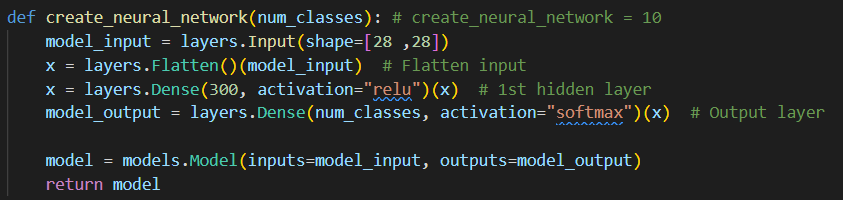
\includegraphics[width=8cm]{imgFolder/create-neural-network-code.png}
\end{figure}

Flatten Layer: This layer flattens the 2D feature maps into a 1D vector,
preparing the data for input into a fully connected neural network.\\\newline
Dense Layers: Fully connected layers that perform classification based on the learned features.
The first dense layer has 300 units with relu activation, enabling the network to learn complex
patterns in the flattened feature vectors.
The second dense layer has 128 units with relu activation, enabling the network to learn complex
patterns in the flattened feature vectors.
The final dense layer has units equal to the number of classes
in the dataset, with softmax activation, which outputs probabilities for each class,
indicating the likelihood of the input image belonging to each class.\\\newline

\code{train-neural-network:}
\\\newline
\begin{figure}[H]
    \caption{Creation of simple neural network model}
    \centering
    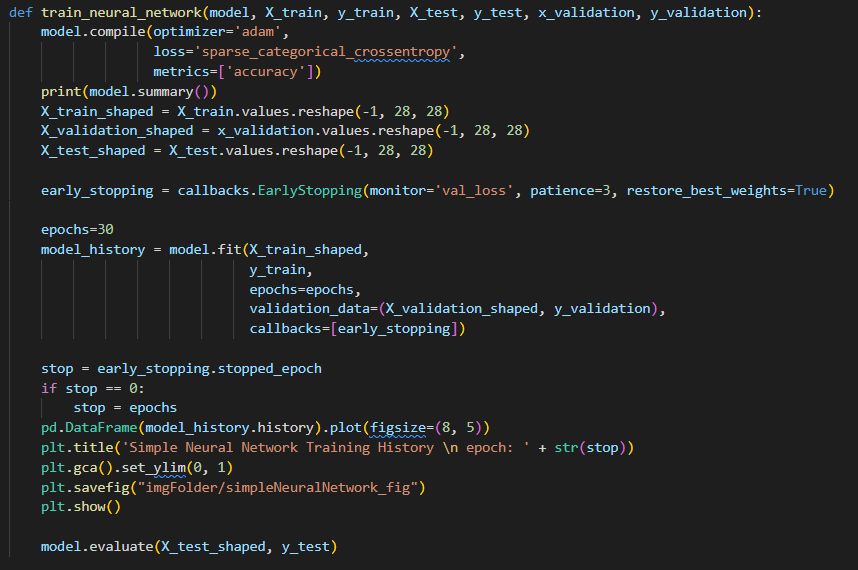
\includegraphics[width=8cm]{imgFolder/train_neural_network-code.png}
\end{figure}
This function prepares the training and test datasets by reshaping them into the format
required for Simple neural network input, constructs the simple neural network model by calling the `create-neural-network` function,
compiles the model and trains the model using the provided training data.
We used early stopping to halt training if the validation loss does not improve for three consecutive epochs,
trying to avoid overfitting.
The training process's history is plotted, showing metrics evolution over epochs.
\newpage

\subsection{CNN Model}
CNN.py code implements a Convolutional Neural Network (CNN) using TensorFlow's Keras API for image classification tasks. It consists of two functions: create-cnn-model and train-cnn-model. The former constructs a CNN model with multiple convolutional and dense layers, along with batch normalization and dropout for regularization. The latter function prepares the training and test datasets, compiles and trains the CNN model, and visualizes the training history, showcasing metrics evolution over epochs (as we saw in figure 14). Early stopping is used to prevent overfitting by halting training if validation loss does not improve for three consecutive epochs.\\\newline
\code{create-cnn-model:}

\begin{figure}[H]
\caption{Creation of the CNN model}
\centering
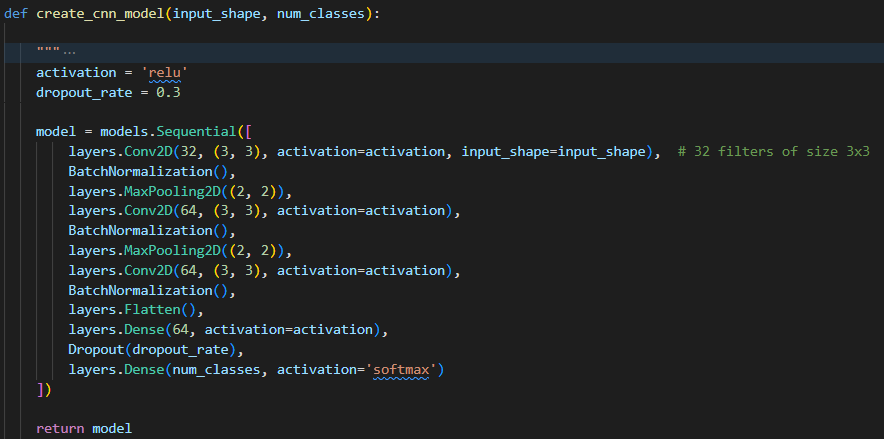
\includegraphics[width=8cm]{imgFolder/create_cnn_model.png}
\end{figure}
\text{ }\\
Convolutional Layers: These layers apply a convolution operation to the input image,
extracting various features through filters.
The activation function used is ReLU,
which introduces non-linearity into the model, enabling it to learn complex patterns.\\\newline
Batch Normalization: This technique is used to improve the training stability and speed
by normalizing the inputs of each layer.\\\newline
MaxPooling Layers: Max pooling reduces the spatial dimensions of the feature maps,
effectively downsampling the input.
It retains the most important features while reducing computational
complexity and preventing overfitting.\\\newline
Flatten Layer: This layer flattens the 2D feature maps into a 1D vector,
preparing the data for input into a fully connected neural network.\\\newline
Dense Layers: Fully connected layers that perform classification based on the learned features.
The first dense layer has 64 units with ReLU activation, enabling the network to learn complex
patterns in the flattened feature vectors.
The final dense layer has units equal to the number of classes
in the dataset, with softmax activation, which outputs probabilities for each class,
indicating the likelihood of the input image belonging to each class.\\\newline
Dropout: This layer was added to prevent overfitting.
It works by randomly setting a fraction of input units to zero during training,
which helps to prevent the network from relying too much on specific neurons
and encourages it to learn more robust features.
We've defined a Dropout layer with a dropout rate of 0.2.
This means during training, ${20\%}$ of the input units to the Dropout layer will be randomly set to zero.\\\newline

\code{train-cnn-model:}\\\newline
This function prepares the training and test datasets by reshaping them into the format
required for CNN input, constructs the CNN model by calling the `create-cnn-model` function,
compiles the model and trains the model using the provided training data.
We used early stopping to halt training if the validation loss does not improve for three consecutive epochs,
trying to avoid overfitting.
The training process's history is plotted, showing metrics evolution over epochs.
\begin{figure}[H]
\caption{Training of the CNN model}
\centering
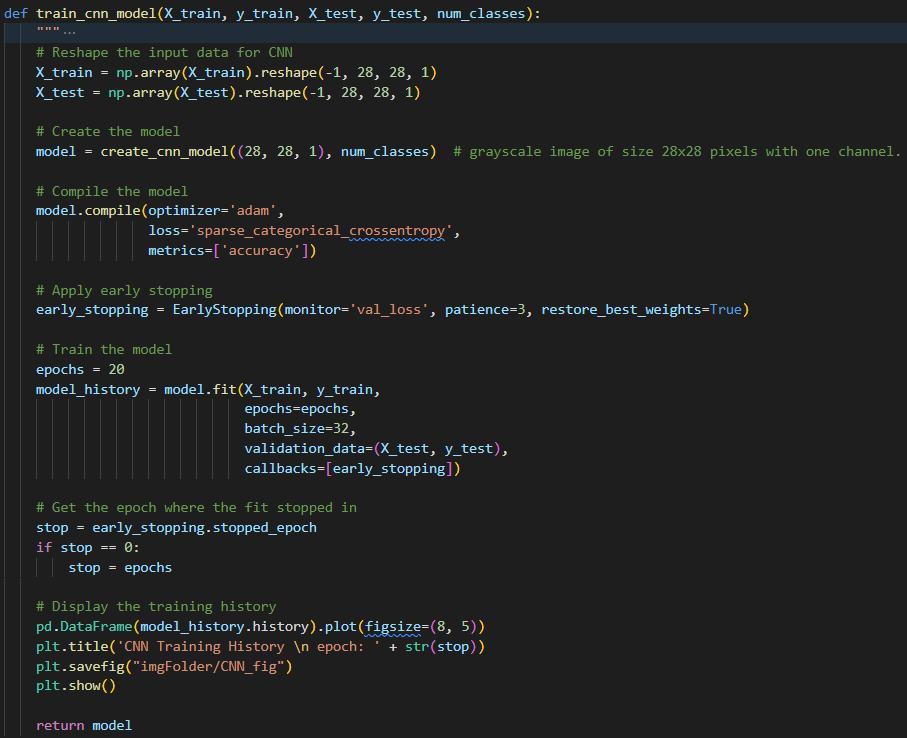
\includegraphics[width=8cm]{imgFolder/train_cnn_model.png}
\end{figure}
% \newpage
\section{Conclusion}
In this study, various machine learning models were evaluated for the classification of fashion items using the Fashion-MNIST dataset. Comparison of traditional algorithms like Logistic Regression and Multi-Layer Perceptron with advanced techniques such as Softmax Regression, Convolutional Neural Networks (CNNs), and Simple Neural Networks revealed that the CNN architecture consistently outperformed others in accuracy and loss reduction. Through systematic exploration of hyperparameters, the optimized CNN model demonstrated superior performance, highlighting the efficacy of deep learning techniques for image classification tasks. These findings contribute valuable insights for applications in e-commerce, retail, and computer vision domains.
\end{document}